\documentclass[a4paper,11pt]{article}
\usepackage[hidelinks]{hyperref}
\usepackage{graphicx}
\usepackage[utf8]{inputenc}
\usepackage[T1]{fontenc}
\usepackage[portuguese]{babel}
\usepackage{indentfirst}
\usepackage{mathtools}
\date{\today}
\author{João Calhau - 31621 \\ André Figueira - 31626} %ver depois se uso \and ou \\
\title{{\bf Universidade de Évora}\\Arquitetura de Sistemas e Computadores\\Relatório do Trabalho Prático}

\begin{document}

 % Primeira Página:
\maketitle
\begin{figure}[ht!]
\centering

\includegraphics[width=90mm]{universidade}
\label{overflow}
\end{figure}

\newpage

%Segunda Página
\tableofcontents

\newpage

% Terceira Página
\section{Objectivo}

\indent Pretende-se com este trabalho desenvolver um conjunto de funções em assembly Mips para detecção de contornos em imagems a cores. Dada uma imagem RGB, o resultado final iria ser uma imagem em tons de cinzento, com fundo branco e com traços escuros nos locais onde existem contornos na imagem original.

\subsection{Como é que este objectivo vai ser atingido?}

\indent Este objectivo vai ser atingido através de várias funções criadas que irão dividir o problema em várias funções de forma a facilitar a resolução. Durante a construção destas funções notam-se também o chamamento de funções auxiliares para dividir o problema numa forma mais detalhada.

\begin{figure}[ht!]
\centering
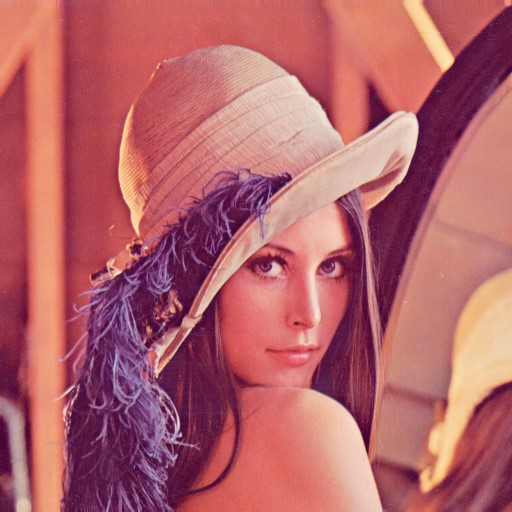
\includegraphics[width=40mm]{Lena512x512}
\caption{Lena}
\label{overflow}
\end{figure}

\begin{center}
$\downarrow$
\end{center}

\begin{figure}[ht!]
\centering
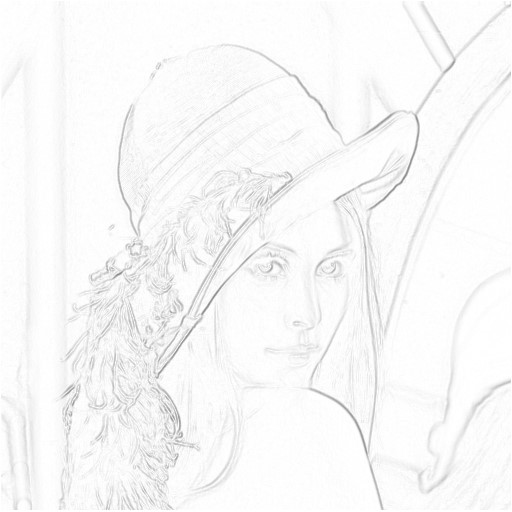
\includegraphics[width=40mm]{Lena(final)}
\caption{Lena (Final)}
\label{overflow}
\end{figure}


\newpage

% Quarta pagina
\section{Descrição}
\subsection{Esquema}

\begin{figure}[ht!]
\centering
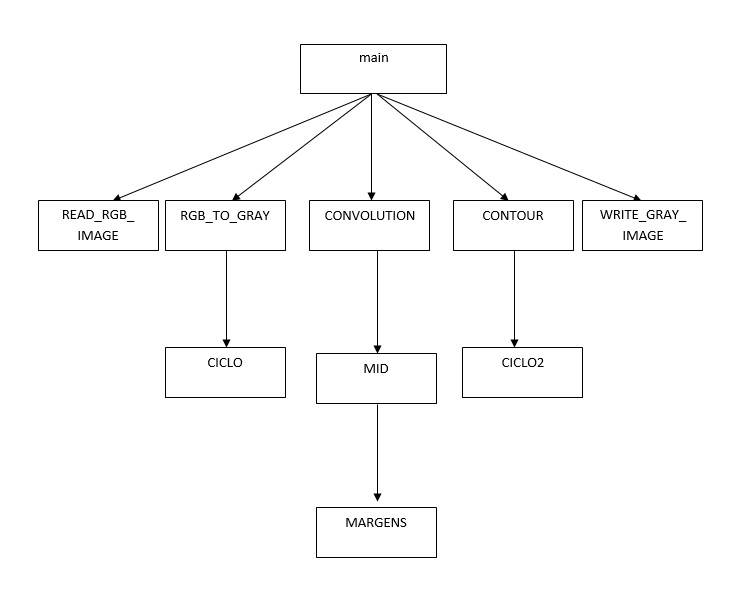
\includegraphics[width=160mm]{esquema}
\label{overflow}
\end{figure}

\newpage
\subsection{Conversão da imagem para formato RGB}

\indent Usando a linha de comando {\bf sudo apt-get install ImageMagick} obtém-se uma ferramenta capaz de conseguir atingit o objectivo de conversão para RGB.
O Próximo passo consiste em abrir o terminal e na directoria, onde se encontra a imagem que irá ser utilizada, usar a linha de comando {\bf convert example.tiff example.rgb}, sendo {\bf .tiff} um formato de imagem (podendo ser este qualquer outro, por exemplo {\bf .jpg}) como resultado obtemos uma imagem em formato RGB pronta a ser utilizada pelo programa.

\newpage

% Quinta Pagina
\subsection{O procedimento}

\indent A explicação do procedimento é feita em duas partes, a primeira é em relação ao {\bf .data segment} e a outra em ralação ao {\bf .text segment}.

\subsubsection{O .data segment}

\indent É nesta região da memória em que se encontram todos os buffers utilizados, contendo também localização do ficheiro de input e output, juntamente com as respectivas directorias. Como se pode ver pela figura 3:
\newline

\begin{figure}[ht!]
\centering
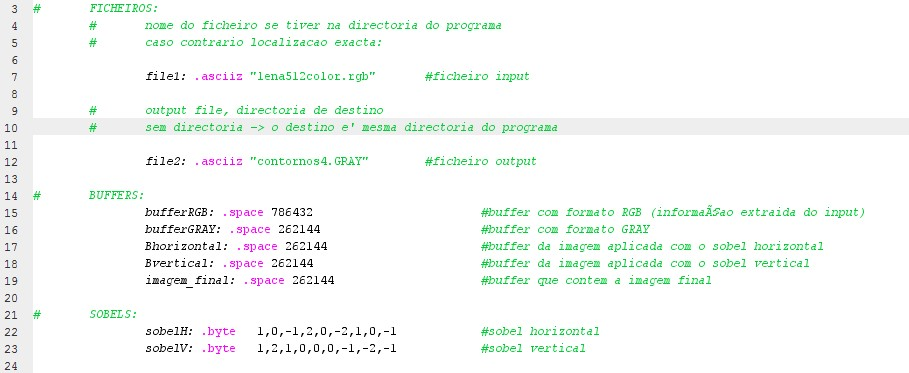
\includegraphics[width=150mm]{imagem}
\caption{.data segment}
\label{overflow}
\end{figure}

\newpage

%Sexta Página
\subsubsection{O .text segment}

\indent Neste segmento é one se encontra a parte do código que irá resolver o problema de detectar os contornos da imagem. Para tal, o .text segment está dividido em vários {\bf branches}.
\newline

O {\bf branch} mais importante neste programa é sem dúvida o {\bf main},

\begin{figure}[ht!]
\centering
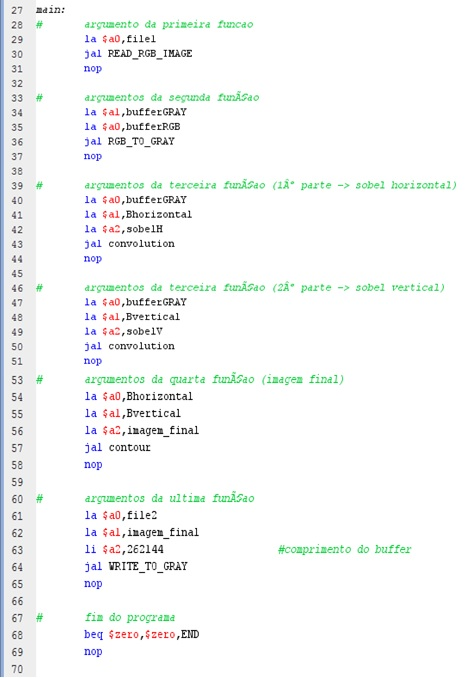
\includegraphics[width=90mm]{imagem1}
\caption{Parte 'main' do .text segment}
\label{overflow}
\end{figure}

Este branch é o {\bf branch central}, a partir deste tudo se controla, pois é este que efectua o chamamento de todas as outra funções que irão aingir, no fim, o objectivo desejado.

\newpage

\noindent{\bf 1ª Função:}
\newline
\newline
\indent O branch {\bf READ\_RGB\_IMAGE}, recebe como argumento o ficheiro de input e transfere o conteúdo RGB para um buffer ({\bf bufferRGB}) em memória.

\begin{figure}[ht!]
\centering
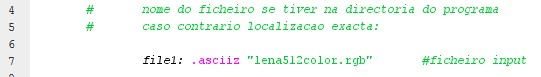
\includegraphics[width=100mm]{imagem2}
\caption{Ficheiro de input}
\label{overflow}
\end{figure}

\noindent{\bf 2ª Função:}
\newline
\newline
\indent O branch {\bf RGB\_TO\_GRAY}, recebe como argumentos dois buffers, um buffer que contem o {\bf bufferRGB} e um buffer vazio ({\bf bufferGRAY}), esta função efectua uma chamada de uma função auxiliar {\bf CICLO} que irá percorrer um ciclo {\bf while} que utilizando as instruções {\bf lbu} ({\bf load byte unassygned}), pois não é necessário a extensão de sinal, chama 3 bytes (ou seja um pixel em RGB) seguidos do bufferRGB que são aplicados na fórmula:
\newline
\begin{center}
{\bf I = 0.30R + 0.59G + 0.11B}
\end{center}

Esta fórmula serve para nos fornecer o valor em gray do pixel correspondente à posição do pixel da imagem em formato RGB. Usando a instrução {\bf sb} ({\bf store byte}) guarda-se o resultado da fórmula no {\bf bufferGRAY}, em seguida basta incrementar os contadores e buffers para seguirem para o próximo pixel. Este ciclo é repetido {\bf 786432 + 3} (+3 bytes, ou seja, mas um pixel, para não terminar antes de completar o ultimo pixel). Quando terminar, executa {\bf jr \$ra}, que volta para a função {\bf RGB\_To\_GRAY} e a partir dai volta para a main pronta para passar para a proxima função.
\newline
O resultado da imagem deverá ser algo como:

\begin{figure}[ht!]
\centering
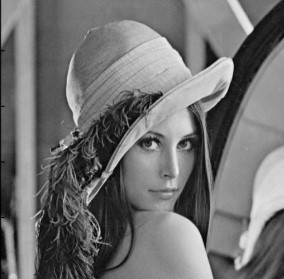
\includegraphics[width=40mm]{Lena(Gray)}
\caption{Lena depois de aplicado a função RGB\_TO\_GRAY}
\label{overflow}
\end{figure}

\newpage

\noindent{\bf 3ª Função:}
\newline
\newline
\indent A função {\bf convolution}, é a única que é chamada duas vezes a partir do {\bf main}, isto porque o exige visto que a imagem guardada no bufferGRAy tem e ser aplicada com sobel, vertical e horizontal. Esta funcção tem dois chamamentos de funções auxiliares, visto que a {\bf MID} (a principal) percorre o interior da imagem à excepção da primeira e ultima linha e das margens. Esta função usando a instrução {\bf lbu (load byte unassygned)} chama um pixel (por ordem de posição no bufferGRAY) e usando a formula:

\begin{figure}[ht!]
\centering
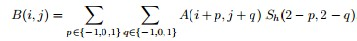
\includegraphics[width=90mm]{formula}
\caption{Formula fornecida pelo docente}
\label{overflow}
\end{figure}

é usada em conjunto com as matrizes (1ª chamada da função convolution utiliza a matriz sobel horizontal e na 2ª a matriz sobel vertical):

\begin{figure}[ht!]
\centering
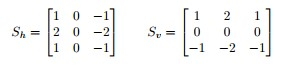
\includegraphics[width=70mm]{matrizes}
\caption{matrizes Sobel vertical (Sv) e horizontal (Sh)}
\label{overflow}
\end{figure}

\begin{center}
(Utilizando também um load byte mas desta vez apenas lb, porque é necessário haver extensão de sinal, valor negativo)
\end{center}
Permite então através de um ciclo {\bf while} obter o valor do dito pixel aplicado com sobel e após ter sido utiizada a formula do somatório usar a seguinte formula:

\begin{figure}[ht!]
\centering
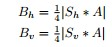
\includegraphics[width=35mm]{formula2}
\caption{Outra formula fornecida pelo docente}
\label{overflow}
\end{figure}

\newpage

Usando a instrução {\bf sb (store byte)} guarda o resultado num novo buffer (1ª chamada no main - bhorizontal, 2ª chamada no main - bvertical). Repetindo o cilco {\bf 261632 -2} (-2 para conseguir fazer o ultimo pixel da penúltima linha e não terminar antes de o fazer).
\newline

Esta fórmula apresenta um problema visto que não está definida para as margens, por isso é que o ciclo tem -512 ao valor original de 262144, para não percorrer a ultima linha (ficando assim a prento por default), e o contador (começando no 1) do ciclo começa em 514 para meter por default a primeira linha mais o primeiro elemento da segunda linha a 0 e começando na posição seguinte (posição 514).
\newline

Por isso foi criada uma função auxiliar {\bf MARGENS} com o propósito de as detectar. Esta função é chamada pela função {\bf MID} quando o contador \$t0 cumpre uma restrição, esta restrição consiste em, o contador se for igual ao tamanho do valor da linha irá fazer com que avance 2 pixéis no contador e posições nos buffers para a frente:

\begin{figure}[ht!]
\centering
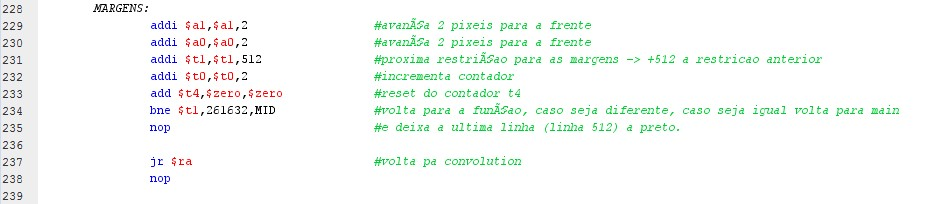
\includegraphics[width=150mm]{imagem3}
\caption{Função {\bf MARGENS}}
\label{overflow}
\end{figure}

Se o valor da restrição for igual ao valor da penúltima linha, a função volta para a função convolution e daí volta para a main.
Em seguida será repetir esta função outra vez, para aplicar o sobel vertical à imagem.
\newline
\newline
{\bf Nota:} visto que existe chamamento de função dentro de função é necessário guardar o valor do registo {\bf \$ra} usando a pilha para se conseguir voltar para a função {\bf main} e continuar o programa e não entrar num cilco infinito.

\newpage

O resultado deverá ser algo como:

\begin{figure}[ht!]
\centering
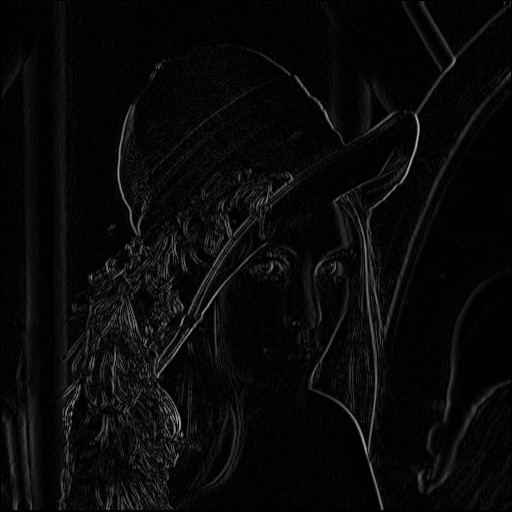
\includegraphics[width=70mm]{Lena(SHorizontal)}
\caption{Lena com o Sobel Horizontal aplicado}
\label{overflow}
\end{figure}

\begin{figure}[ht!]
\centering
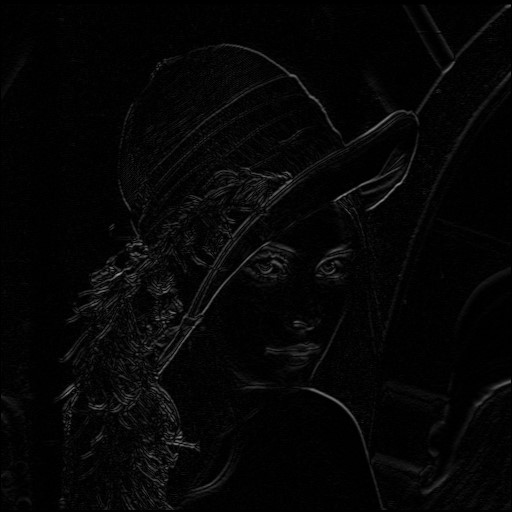
\includegraphics[width=70mm]{Lena(SVertical)}
\caption{Lena com o Sobel Vertical aplicado}
\label{overflow}
\end{figure}

\newpage

\noindent{\bf 4ª Função:}
\newline
\newline
\indent A função {\bf contour} recebe como argumentos os dois buffers aplicados com os sobels vertical e horizontal (bhorizontal e bvertical), efectua uma chamada de uma função auxiliar {\bf CICLO2} que através de um ciclo while fazendo a soma de cada ponto, aplicando a seguinte fórmula:

\begin{figure}[ht!]
\centering
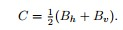
\includegraphics[width=35mm]{formula3}
\caption{Ainda outra formula fornecida pelo docente}
\label{overflow}
\end{figure}

E depois aplicando a seguinte formula para inverter as cores a cada ponto:

\begin{figure}[ht!]
\centering
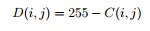
\includegraphics[width=45mm]{formula4}
\caption{Ainda outra formula fornecida pelo docente}
\label{overflow}
\end{figure}

Através destas duas formulas guarda-se o resultado no buffer {\bf imagem\_final}.
\newline
\indent Para optimização de código escolheu aplicar-se directamente durante o ciclo while às duas formulas. Permitindo assim quando se efectua o chamamento dos pontos dos dois buffers (bhorizontal e bvertical) usando a instruçãp {\bf lb} para que o ponto que entrasse no buffer imagem\_final fosse o ponto final sem necessidade de passos adicionais. Ao terminar executa o {\bf jr \$ra} que volta para a função {\bf contour} e dai volta para a função main.
\newline

\noindent {\bf 5ª Função:}
\newline
\newline
\indent O branch {\bf WRITE\_TO\_GRAY}, tem o único propósito de escrever num ficheiro (output), que neste caso é transferir a informação contida no buffer {\bf imagem\_final} para o ficheiro output. Ao terminar executa {\bf jr \$ra} onde volta para main e termina o programa.

\begin{figure}[ht!]
\centering
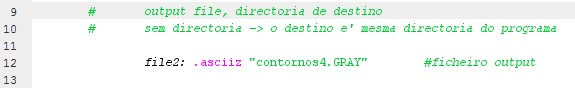
\includegraphics[width=150mm]{imagem4}
\caption{Ficheiro de Output}
\label{overflow}
\end{figure}


\newpage
\subsection{Conversão de formato .GRAY para formato .jpg (exemplo)}

Usando a linha de comando na directoria da imagem final (5º Passo), {\bf convert -size 512x512 -depth 8 imagem.gray imagem.jpg} é nos permitido converter a imagem para a seguinte:

\begin{figure}[ht!]
\centering
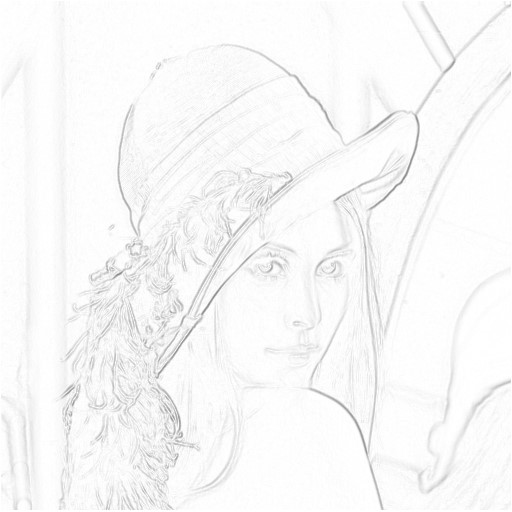
\includegraphics[width=110mm]{Lena(final)}
\caption{Lena (Resultado final)}
\label{overflow}
\end{figure}

\newpage
\section{Curiosidades}

O Programa executa 39 017 632 instruções, tendo em conta que o processador tem 2.13 Ghz, excuta o programa em 0.0183181371 segundos
\newline

A imagem presente no enunciado do trabalho não se parece com a demonstrada anteriormente, portanto após varios testes, descobriu-se que para ficar igual à imagem aprensentada no enunciado tinha de haver uma modificação na formula:

\begin{figure}[ht!]
\centering
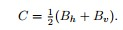
\includegraphics[width=40mm]{formula3}
\label{overflow}
\end{figure}

Esta modificação consiste apenas em multiplicar-se a formula acima por 2, a imagem, assim, seria:

\begin{figure}[ht!]
\centering
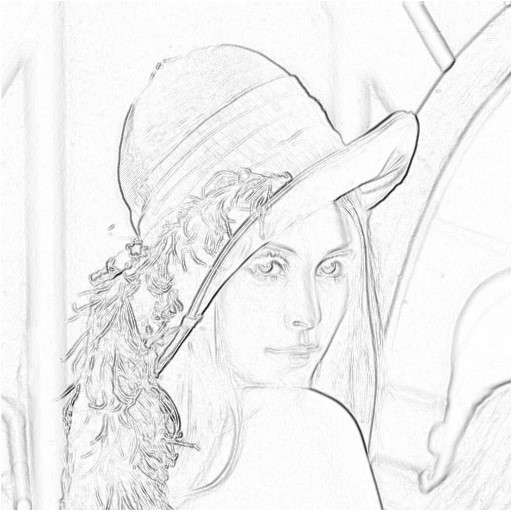
\includegraphics[width=100mm]{Lena(final2)}
\caption{Lena com a formula modificada aplicada}
\label{overflow}
\end{figure}

Que por si, é muito semelhante à do enunciado.

\newpage
\section{Conclusão}

No final do programa podemos concluir que foi um sucesso, o programa faz o que tem a fazer sem erros ou bugs detectados. Conclui-se também que através deste trabalho ao aplicar todos os conhecimentos adquiridos em Arquitectura de Sistemas e Computadores contribuiu para um maior conhecimento e entendimento.

\newpage
\section{Bibiografia}

\noindent {\bf Bibliografia usada:}
\newline

\noindent {\bf Syscalls}
\newline
\noindent \href{http://courses.missouristate.edu/kenvollmar/mars/help/syscallhelp.html}{http://courses.missouristate.edu/kenvollmar/mars/help/syscallhelp.html}
\newline

\noindent {\bf ImageMagick}
\newline
\noindent \href{http://www.imagemagick.org/}{http://www.imagemagick.org/}
\newline

\noindent {\bf obel Operator}
\newline
\noindent \href{http://en.wikipedia.org/wiki/Sobel_operator}{http://en.wikipedia.org/wiki/Sobel\_operator}
\newline

\end{document}
